\chapter{Stellar konsenzus protokol}

\label{kap:stellar}

V tejto časti si predstavíme protokol \cite{mazieres2015stellar}, ktorý bude
spĺňať všetky popísané požiadavky v kapitole vyššie a bude zaručené,
že všetky správne fungujúce uzly sa dohodnú na rovnakej hodnote.

Každý uzol si bude udržiavať svoju kópiu blokovej reťaze. Jednu transakciu (a
metadáta o nej) v blokovej reťazi budeme nazývať \textit{blok}.
Cieľom tohto konsenzus protokolu teda je aby sa celá sieť vždy dohodla
na obsahu nového bloku a všetky uzly si ju mohli zapísať do svojej
blokovej reťaze. 
Budeme tiež predpokladať, že každý uzol dodržujúci protokol nikdy nebude tvrdiť
dve protichodné tvrdenia.

\section {Kvórum a typy uzlov}

Keď sa uzol dozvie od dostatočného množstva iných uzlov informáciu, uverí jej a
bude predpokladať, že žiadny uzol dodržujúci protokol nikdy nebude tvrdiť nič
protichodné.
Takúto množinu uzlov pre uzol \textit{v} budeme nazývať kvórový rez. Keďže
sa nám po čase môže stať, že niektoré uzly zlyhajú, dovolíme mať každému vrcholu
viac kvórových rezov.

\paragraph {Stellar systém} budeme nazývať
dvojicu $<\textbf{V},\textbf{Q}>$ kde $\textbf{V}$ bude zoznam uzlov a $\textbf
{Q}$ bude funkcia priradzujúca uzlom \textit{kvórové rezy}.
\newline
Presnejšie:
$$\textbf{Q} : \textbf{V} \to 2^{2^V} \setminus \emptyset \quad
\forall v \in \textbf{V}, \forall q \in \textbf{Q}(v), v \in q$$


Teda každý vrchol obsahuje sám seba v každom svojom kvórovom reze.
Kvórový rez bez vrcholu, ktorému prislúcha budeme nazývať \textit{vlastný kvórový rez}.

\paragraph {Kvórum} je množina uzlov $U \subseteq V$ v
Stellar systéme práve vtedy keď $U \neq \emptyset$ a $U$ obsahuje kvórový rez pre
každý jeho prvok, teda $\forall v \in \textbf{U} \: \exists q \in \textbf{Q}
(v)$,
že $q \subseteq U$

\begin{flushleft}
Kvórum je množina uzlov dostatočná na dosiahnutie konsenzu. Totiž táto množina obsahuje
pre každý svoj prvok kvórový rez, ktorý ho dokáže presvedčiť.
Na obrázku \ref{obr:kvorum} je znázornená jedna možnosť ako si uzly mohli navoliť
kvórové rezy.
Všimnime si, že napríklad množina $\{v_2, v_3, v_4\}$ je síce kvórový rez uzlu
$v_4$, ale kvórum netvorí, keďže neobsahuje jediný kvórový rez $v_2$.
Naopak množina uzlov $\{v_1, v_2, v_3\}$ je kvórový rez uzlov $v_1, v_2, v_3$ a
teda aj tvorí kvórum.

\begin{figure}
\centerline{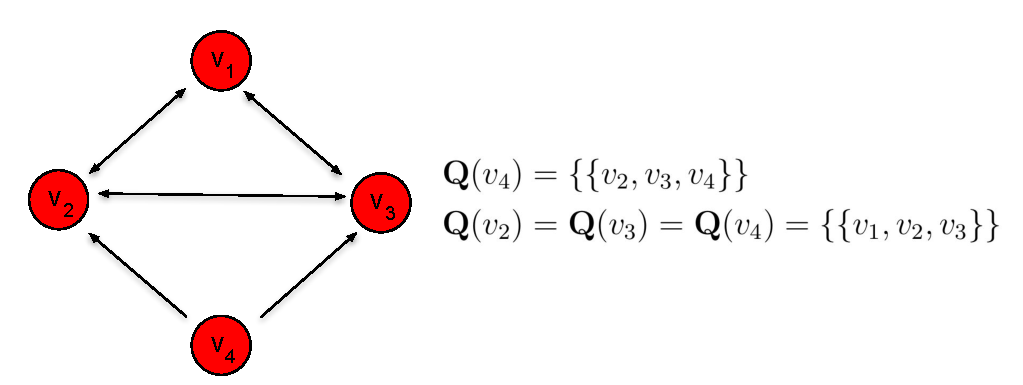
\includegraphics[width=0.8\textwidth]{images/kvorum.pdf}}
\caption[Príklad siete]{Príklad volenia kvórových rezov od uzlov} \label{obr:kvorum}
\end{figure}

\end{flushleft}

Uzly budeme rozdeľovať do dvoch hlavných skupín -- na uzly držiacie sa protokolu a
nedržiace sa protokolu. Medzi uzly nedodržiavajúce protokol zaraďujeme buď
Byzantíncov (napríklad nepriateľ sa zmocnil uzlu) alebo uzly, ktoré akýmkoľvek
spôsobom zlyhali.
Cieľom protokolu je aby uzly dodržujúce protokol dosiahli konsenzus. Toto vieme
popísať dvomi vlastnosťami.

\paragraph {Bezpečnosť} Množina uzlov v Stellar systéme je \textit{bezpečná}, ak žiadne
dva uzly z nich neschvália pre jeden konkrétny blok iné hodnoty. Teda nebudú mať
rôzne verzie transakčnej histórie.

\paragraph {Životaschopnosť} Množina uzlov v Stellar systéme je \textit{životaschopná},
ak vie schvaľovať nové bloky do svojej blokovej reťaze, bez potreby spolupráce
zlyhaných uzlov. Rovnako vieme definovať \textit{životaschopný} uzol.

\vspace{4mm}
Obe tieto definície sú len popisom vlastností, ktoré chceme dosiahnuť.
Neskôr v práci si aj zadefinujeme ako vieme zistiť, kedy \textit{Stellar systém}
tieto vlastnosti má, už len z popisu samotného systému.

Teraz uzly dodržujúce protokol rozdelíme do troch skupín. Uzly, ktoré budú porušovať
podmienku bezpečnosti budeme označovať ako \textit{divergentné}. Všimnime si, že
toto je veľmi ťažké exaktne definovať, keďže nevieme, ktorá bloková reťaz,
je tá správna a ktorá divergovala (každý uzol si totiž drží vlastnú kópiu a
povedať objektívnu pravdu je náročné).
Avšak tento pojem budeme potrebovať len na intuitívne pochopenie fungovania siete
a teda s predstavou, že \textit{divergentný} uzol, je taký uzol, ktorý schválil
niečo iné ako tie \uv{dobré} uzly, si plne vystačíme.

Uzly, ktoré síce sú bezpečné ale nie sú životaschopné zase budeme označovať ako
\textit{zablokované}. A nakoniec uzly, ktoré sú aj bezpečné aj životaschopné budeme
označovať ako \textit{korektné}.

Všimnime si, že aj uzly dodržujúce protokol môžu byť divergentné, stačí, že
hlasovaním spolu s Byzantíncami sa im poškodila bloková reťaz. Práve takýmto
situáciám sa bude Stellar protokol snažiť vyhnúť.
Vizualizáciu katogorizácie uzlov môžeme vidieť na obrázku \ref{obr:typy_uzlov}.

\begin{figure}
\centerline{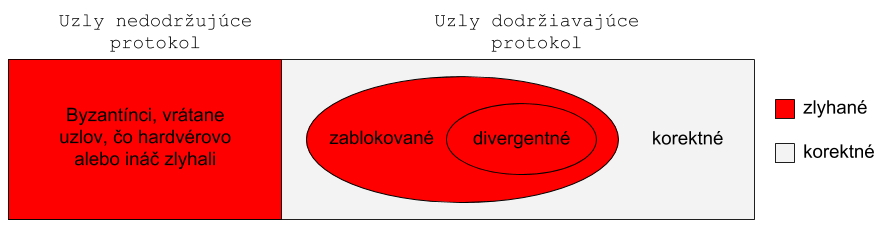
\includegraphics[width=0.8\textwidth]{images/rozdelenie_uzlov}}
\caption[Kategorizácia uzlov]{Rozdelenie uzlov do kategórie podľa schopnosti
zúčastňovať sa na konsenze} \label{obr:typy_uzlov}
\end{figure}

\section {Vlastnosti kvór a uzlov}

Keby si uzly určovali svoje kvóra úplne ľubovoľne, sieť by vôbec nemusela byť
prepojená a teda by mohla byť divergentná. Preto budeme požadovať aby kvóra
spĺňali niektoré vlastnosti.

\paragraph {Prienik kvór} Stellar systém má prienik kvór práve vtedy ak každá
dvojica kvór má aspoň jeden spoločný uzol.

\begin{figure}
\centerline{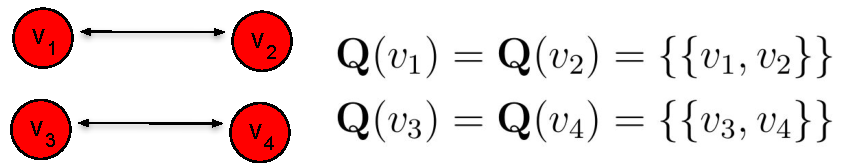
\includegraphics[width=0.8\textwidth]{images/prienik_kvor.pdf}}
\caption[Príklad siete bez prieniku kvór]{Sieť bez prieniku kvór môže
divergovať} \label{obr:prienik_kvor} \end{figure}

\vspace{4mm}
Na obrázku \ref{obr:prienik_kvor} môžeme vidieť príklad siete bez prieniku kvór.
Disjunktné množiny $\{v_1, v_2\}$ a $\{v_3, v_4\}$ sú kvóra bez prieniku. Takže
tieto množiny sú samé o sebe schopné schvaľovať bloky a predlžovať blokovú
reťaz.
Keďže ale nemajú prienik nemusia schváliť rovnaký blok a teda sieť bude
divergovať.

Teraz si definujme operáciu mazania množiny uzlov zo Stellar systému.

\paragraph {Operácia zmaž} Ak máme Stellar systém $<\textbf{V},\textbf{Q}>$ a
zmažeme z neho množinu uzlov $B \subseteq V$, dostaneme systém $<\textbf{V},
\textbf{Q}>^B \: = \: <\textbf{V} \setminus B,\textbf{Q}^B>$, kde $\textbf{Q}^B
= \{q \setminus B \: | \: q \in \textbf{Q}(v)\}$.

\vspace{5mm}
Takto si ľahko vieme zúžiť systém na množinu uzlov, ktoré chceme ďalej uvažovať
a pomocou toho analyzovať odolnosť siete aj po prehlásení niektorých uzlov
za nedôveryhodné. Ako sme si už hovorili tak aby bolo kvórum schopné dosiahnuť
konsenzus a budovať rovnakú blokovú reťaz, musí mať prienik kvór. Avšak ak je
tento prienik práve byzantínsky uzol, tak naša sieť bude aj tak divergentná,
keďže práve on môže poslať správu jednému kvóru že hlasoval \textit{za} schválenie
nového bloku a druhému poslať správu, že hlasoval \textit{proti} a oba môžu schváliť
protichodné tvrdenia. Preto aby naša sieť bola odolná aj voči zlyhaniam niektorých
uzlov, bude musieť mať väčšie prieniky kvór.
Pre lepšie popísanie tejto problematiky si dodefinujeme \textit{nepotrebné množiny}.
Budeme chcieť mať sieť rozloženú tak, aby všetky zlyhané uzly boli v
nepotrebnej množine a teda sieť bola schopná prijímať konsenzus aj bez nich.

\paragraph {Nepotrebná množina} Ak máme Stellar systém $<\textbf{V},
\textbf{Q}>$, tak množina uzlov $B$ je nepotrebná práve vtedy keď
\begin{itemize}
\item  $<\textbf{V}, \textbf{Q}>^B$ má prienik kvór
\item  $\textbf{V} \setminus B$ je $\pmb{\emptyset}$ alebo kvórum v $<
\textbf{V}, \textbf{Q}>$
\end{itemize}

Prvá podmienka chráni sieť pred divergenciou, ktorú by mohli spôsobovať uzly z
$B$, tým že by schvaľovali protichodné tvrdenia. Tým, že prienik kvór ostane
zachovaný aj keď uzly z $B$ uvažovať nebudeme, sieť naozaj divergovať nebude.
Ak sieť danú podmienku spĺňa zvykneme hovoriť, že sieť má prienik kvór aj
\textit{napriek množine B}.

Naopak druhá podmienka zachováva životaschopnosť siete bez ohľadu na uzly z $B$,
keďže zaručuje, že aj bez uzlov z $B$ vedia ostatné uzly schvaľovať nové bloky.
Splneniu tejto podmienky zvykneme hovoriť životaschopnosť aj
\textit{napriek množine B}.

Čo si môžeme všimnúť je, že uzly musia balansovať vo veľkosti vyberaných kvórových
rezov. Keď si totiž uzly vyberú veľké kvórové rezy, tak vzniknú veľké kvóra.
Toto potom vedie k veľkým prienikom kvór (musí zlyhať veľa uzlov na
zničenie prieniku kvór), čo nám zaručuje malú šancu nepriateľa zničiť bezpečnosť
siete. Avšak oveľa ľahšie ohrozí jej životaschopnosť, keďže zlyhanie už len
málo uzlov ovplyvní veľa kvór. Podobne naopak pri malých kvórach vzniknú menšie
kvórové prieniky, čo zjednoduší nepriateľovi ohroziť bezpečnosť siete, avšak
bude musieť zlyhať viac uzlov aby to ohrozilo životaschopnosť siete
(aby zlyhali uzly v čo najviac kvórach).
Uzly v sieti teda musia nájsť balans pre čo najväčšiu obranyschopnosť siete.

Na záver tejto podkapitoly sme už teda pripravený si definovať \textit{bezpečnosť}
a \textit{životaschopnosť} siete na základe vlastností konkrétneho
\textit{Stellar systému}, aby zároveň boli splnené definície a očakávania
spomenuté na začiatku kapitoly.

\pagebreak

\paragraph {Bezpečnosť}
Stellar systém je \textit{bezpečný} práve vtedy keď má prienik kvór.

\paragraph {Životaschopnosť}
Množina uzlov $A$ v Stellar systéme $<\textbf{V}, \textbf{Q}>$ je
\textit{životaschopná}, práve vtedy, keď tento Stellar systém bude životaschopný
aj \textit{napriek množine} $V \setminus A$.

\vspace{5mm}
Vieme si zadefinovať aj \textit{životaschopnosť} uzlu $v$ v Stellar systéme voči
množine $B$. A to tak, že bude musieť mať mať aspoň jeden kvórový rez neobsahujúci
uzol z množiny $B$ (teda bude schopný byť súčasťou niektorého kvóra bez zlyhaných uzlov).

Táto definícia dáva zmysel, keďže ak uzol $v$ nebude životaschopný voči množine $B$,
tak už žiadna množina uzlov obsahujúcich $v$ neobsahujúca žiadny uzol z $B$
nemôže byť životaschopná. Keďže na uzavretie kvóra potrebujeme aj kvórový rez uzlu $v$.

\section {Priebeh schvaľovania bloku}

Schvaľovanie nového bloku prebieha vo viacerých fázach. Počas tohto procesu sa 
z pohľadu každého uzlu môže blok nachádzať v 3 rôznych stavoch -
\textit{neznámy}, \textit{akceptovaný}, \textit{potvrdený}.

Na začiatku schvaľovacieho procesu je pre každý uzol blok \textit{neznámy}.
Počas celého priebehu schvaľovania si uzly vymieňajú správy, na základe ktorých
si môže blok zvýšiť stav bloku (pre daný uzol môže ísť blok len do vyššieho
stavu, teda ak už pre neho bol blok \textit{akceptovaný}, nemôže ho blok
prehlásiť spätne za \textit{neznámy}).
Správy si môžeme predstavovať ako hlasovanie uzlov, či má alebo nemá byť
blok pridaný do blokovej reťaze.
Keď pre každý korektný uzol bude blok \textit{potvrdený}, môžu si ho pridať
do svojej blokovej reťaze.

Uzly si budú meniť stavy bloku na základe správ od uzlov zo svojich kvórových rezov
spomínaných vyššie, avšak detajly presných pravidiel na základe ktorých sa tieto
stavy budú meniť využívať nebudeme.
Preto pre potreby našej práce nepotrebujeme vedieť ako a aké správy si medzi
sebou uzly budú vymieňať.
Plnohodnotne nám bude stačiť intuícia zavedenia kvórových rezov a kvór.

Presnješie detajly Stellar konsenzus protokolu, procesu schvaľovania bloku,
samotné dôkazy, že takéto schvaľovanie vedie ku v praxi plne funkčnej sieti a
napokon aj samotnú implementáciu môže čitateľ nájsť v \cite{mazieres2015stellar}.

\vspace{10mm}
Na záver kapitoly si zhrňme, že naozaj tento protokol spĺňa očakávania predstavené
v podkapitole \ref{kap:theorytobank}.
\\
\\

\begin{itemize}
\item  \textbf{Jedna globálna} -- naša sieť sa naozaj nedelí na žiadne podsiete
a každý uzol môže komunikovať s každým
\item  \textbf{Decentralizovaná} -- každý uzol si drží svoju kópiu blokovej reťaze
a žiadna centrálna kópia neexistuje
\item  \textbf{Nízka latencia} -- uzly dokážu schváliť nový blok len po vymenení si
niekoľkých správ, uzly nepotrebujú robiť žiadnu výpočtovo náročnú prácu
\item  \textbf{Otvorené členstvo v sieti} -- pridať sa do siete vie ktokoľvek, stačí
sa pripojiť a nastaviť kvórové rezy
\item  \textbf{Otvorené členstvo medzi schvaľovateľmi} -- \uv{schvaľovateľmi} sú
vlastne uzly, ktoré sa nachádzajú v niekoho kvórovom reze. Stačí si teda vybudovať
dôveru medzi ostatnými členmi siete, samotné pravidlá siete nebránia byť schvaľovateľom
\item  \textbf{Flexibilná dôvera} -- každý uzol si určuje sám svoje kvórové rezy a teda
sám určuje komu bude dôverovať
\item  \textbf{Odolnosť voči zlyhaniam} -- ako sme si ukázali toto záleží už na samotnom
systéme, ale pokiaľ si budú uzly rozumne voliť kvórové rezy, bude mať sieť aj túto vlastnosť.
Hodnoteniu odolnosti jednotlivých sietí sa budeme venovať vo zvyšku našej práce
\end{itemize}